Los resultados obtenidos en cada uno de los pasos de este trabajo se detallan en
este capítulo, comenzando por el motor obtenido en la primera iteración de
optimización con el algoritmo genético junto con el modelo geométrico 3D
generado.
%
Luego se muestran los resultados de las flujometrías realizadas a partir del
modelo de CAD, incluyendo las mallas obtenidas para algunos casos seleccionados
y el resultado detallado de algunas de las flujometrías, finalizando con el mapa
de $C_{D}$ obtenido, tanto para el puerto de admisión como para
el puerto de escape.

Por último se presentan los resultados de la segunda ronda de optimización con
el algoritmo genético, en la que se utilizó el mapa de $C_{D}$ obtenido en el
paso previo.

\section{Primera Iteración}
%
La primera optimización se realizó partiendo de una población al azar, con los
coeficientes de descarga constantes de 0,7 y 0,75 para el puerto de admisión y
escape respectivamente.
%
El algoritmo genético se ejecutó durante 20 generaciones con una población de
100 individuos y la función objetivo definida en la
sección~\ref{sec:funcion_objetivo} con los pesos, operadores y
parámetros correspondientes indicados en la Tabla~\ref{tab:config_genetico}.

\begin{table}[h!]
  \centering
  \begin{tabular}{ccc} \toprule
    Parámetro & Valor & Unidad \\ \midrule
    RPMS & $1000\times[1, 2, 3, 4, 5, 6, 7, 8, 9]$ & \\
    Pesos de función objetivo & $(1, 1, 1, 6, 8, 9, 8, 7, 7)$ & \\
    Diámetro mínimo & 0,05 & m \\
    Diámetro máximo & 0,1 & m \\
    Longitud mínima de tubo & 0,5 & m \\
    Longitud máxima de tubo & 2 & m \\
    Ángulo mínimo & 0 & grados \\
    Ángulo máximo & 90 & grados \\
    Separación angular máxima & 70 & grados \\
    Tamaño de población & 100 & - \\
    Tamaño de torneo & 10 & - \\
    Probabilidad de cruza & 0,9 & - \\
    Probabilidad de mutación & 0,5 & - \\
    Cantidad de generaciones & 20 & - \\
    Tamaño de \emph{SALÓN DE LA FAMA} & 1 & - \\ \bottomrule
    \end{tabular}
  \caption{Configuración utilizada.}\label{tab:config_genetico}
\end{table}

% Nota: terminar de agregar la figura
% Para ICESym se utilizaron dos ciclos de simulación, por considerarse que es
% suficientemente preciso para esta primer aproximación.
%
% En la Figura XX se puede ver que a partir de la segunda iteración se obtienen
% buenos resultados, esto se debe a que los datos de partida para la segunda
% iteración, son los resultados de la primer iteración.
%

En la Figura~\ref{fig:ev_primer_op}, donde se representa la evolución de la
población tras iteraciones sucesivas, se observa que se obtuvo rápidamente un
individuo con un puntaje relativamente alto en las primeras iteraciones.
%
El resultado final tiene una aptitud 1.5 veces la aptitud media de la población
de la última generación, siendo los parámetros que definen este candidato los
listados en la Tabla~\ref{tab:resultado_primer_it} y cuyos indicadores se
ilustran en la Figura~\ref{fig:primer_op}.
%
Este motor tiene un rendimiento volumétrico máximo de $\eta_{v} \simeq 0.83$
para 2500 RPM y si bien la función objetivo favorece curvas suaves, se ven dos
picos de rendimiento en la curva, siendo el segundo con $\eta_{v} \simeq 0.79$ a
7500 RPM.

A modo de comparación, en la misma Tabla se presentan las características
geométricas obtenida en trabajos anteriores~\parencite{mrcvc_geom}.

\begin{figure}[h!]
  \centering
  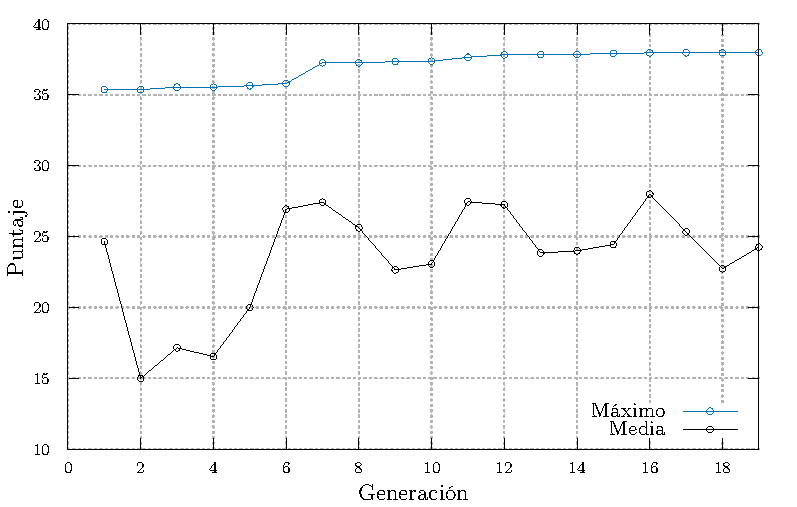
\includegraphics[width=.8\textwidth]{gnuplot/genetico.pdf}
  \caption{Evolución de la población} \label{fig:ev_primer_op}
\end{figure}%
\begin{figure}[h!]
  \centering
  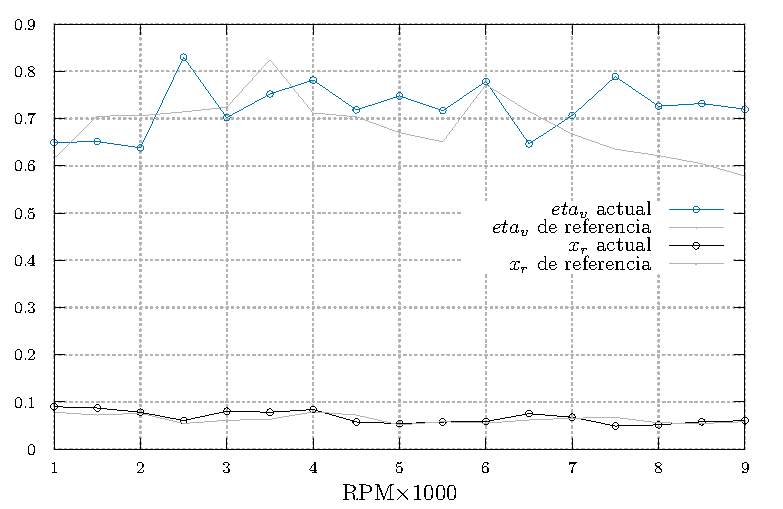
\includegraphics[width=.8\textwidth]{gnuplot/primer-rendimiento.pdf}
  \caption{Rendimiento volumétrico y fracción de gases residuales del motor seleccionado} \label{fig:primer_op}
\end{figure}

% TODO revisar los ángulos de los puertos
\begin{table}[h!]
  \centering
  \begin{tabular}{ccccc} \toprule
    Parámetro & \multicolumn{2}{c}{Admisión} & \multicolumn{2}{c}{Escape} \\ \cmidrule(lr){2-3} \cmidrule(lr){4-5} & Inicial & Final & Inicial & Final \\
    \midrule
    Longitud del tubo [mm]               & 1300   & 519    & 800    & 976  \\
    Diámetro del tubo [mm]               & 70     & 97     & 50     & 81   \\
    Ángulo de apertura del puerto [grad] & 592.93 & 584.05 & 396.87 & 396.69 \\
    Ángulo de cierre del puerto [grad]   & 175.76 & 182.74 & 587.06 & 5.95 \\
    \bottomrule
  \end{tabular}
  \caption{Datos geométricos del mejor candidato}
  \label{tab:resultado_primer_it}
\end{table}


En la Figura~\ref{fig:PoTi_primer_op} se muestran las curvas de potencia y
torque del motor.
%
Como es de esperarse se ve que ambas están directamente condicionadas por el
rendimiento volumétrico, con una potencia al freno máxima de 177 CV a 7500 RPM y
un torque máximo de 191 N.m a\ 2500 RPM.

\begin{figure}[h!]
  \centering
  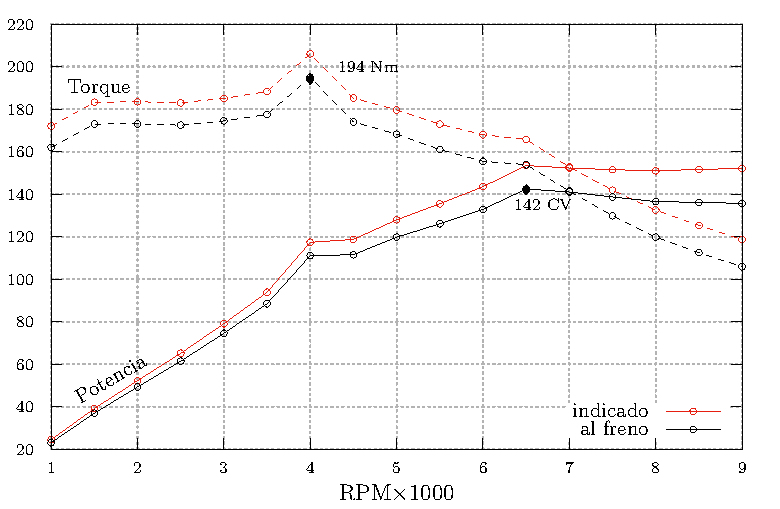
\includegraphics[width=\textwidth]{gnuplot/primer-potencia.pdf}
  \caption{Torque y Potencia de Primera Iteración} \label{fig:PoTi_primer_op}
\end{figure}


\section{Modelo de CAD}
%
A partir de los resultados obtenidos se realizó un modelo de CAD de los puertos
que se ilustra en las Figuras~\ref{fig:motor_cad1} y~\ref{fig:motor_cad2}.
%
Se representó solamente la mitad superior del motor que contiene los puertos
de admisión y escape.
%
Este modelo es paramétrico y permite rotar los componentes del motor para
obtener distintas posiciones del conjunto y así poder generar la geometría a
evaluar con las flujometrías.

% Algunos redondearon las aristas internas incluyendo las paletas y las puntas del rotor para favorecer el proceso de mallado, ya que los bordes agudos pueden ser problmeáticos para el mallador \emph{snappyHexMesh}.

\begin{figure}[h!]
  \centering
  \subfloat[]{
    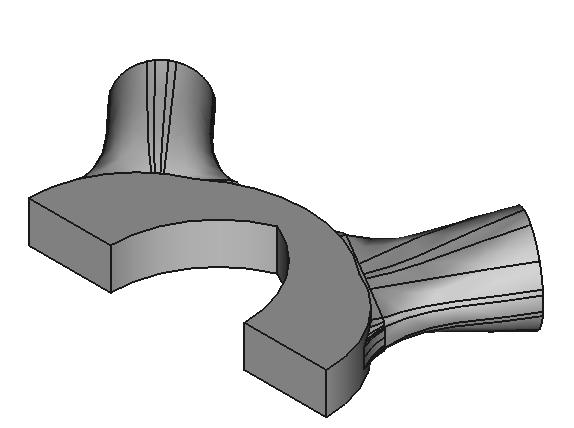
\includegraphics[width=.5\textwidth]{CAD/motor_cad1.png}
  }
  \subfloat[]{
    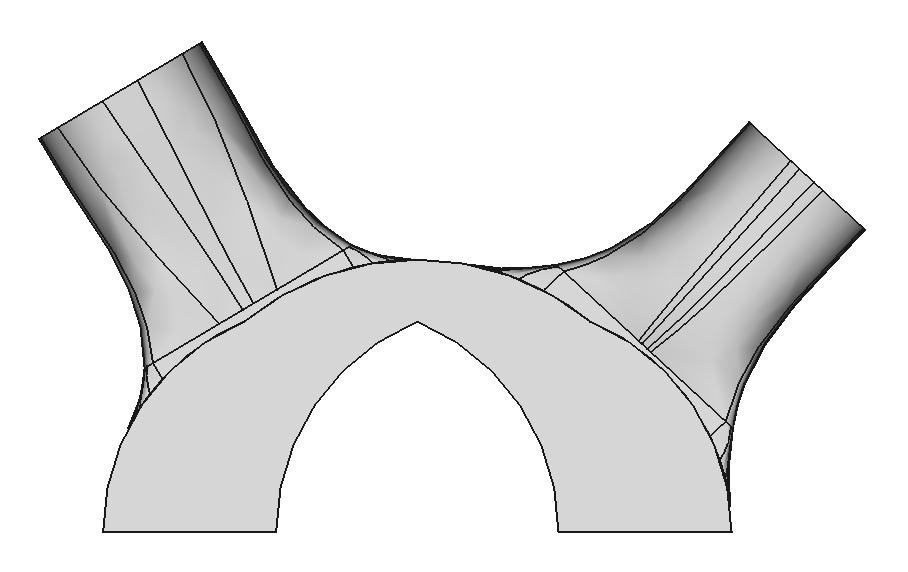
\includegraphics[width=.5\textwidth]{CAD/motor_cad2.png}
  }
  \caption{CAD Primera iteración}\label{fig:motor_cad1}
\end{figure}


\begin{figure}[h!]
  \centering
  \subfloat[Puerto de Admisión]{
    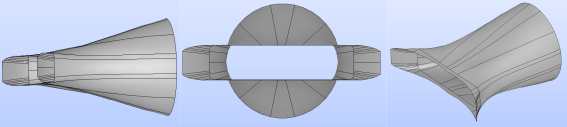
\includegraphics[width=\textwidth]{CAD/vistas_admision.png}
  }
  \hfill
  \subfloat[Puerto de Escape]{
    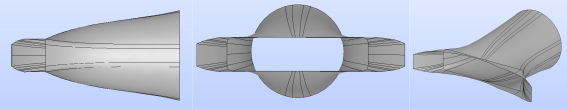
\includegraphics[width=\textwidth]{CAD/vistas_escape.png}
  }
  \caption{CAD Primera iteración (vistas fuera de escala).}\label{fig:motor_cad2}
\end{figure}

La altura del puerto del lado de la cámara se mantuvo en dos tercios de la
altura de la cámara $h_{p} = \frac{2}{3}h_{c}$, manteniendo el eje central de cada
puerto de forma que intersecte el centro del motor con el propósito de eliminar
una variable de la geometría a modelar.
%
El foco de esta etapa de optimización es el diámetro del puerto y el reglaje.
%

%%%%%%%%%%%%%%%%%%%%%%%%%%%%%%%%%%%%%%%%%%%%%%%%%%%%%%%%%%%%%%%%%%%%%%%%%%%%%%%

\section{Flujometrías}

De la primera iteración se obtuvo la geometría y datos operativos del motor, lo
cual permitió representar la curva de diferencia de presión ($\Delta P$) en
función de la alzada ($l_{v}$) de ambos puertos para diferentes velocidades de
giro, identificando los puntos de mayor interés en los cuales realizar las
flujometrías.
%
Los pares $(l_{v}, \Delta P)$ seleccionados para modelar el flujo del puerto se
detallan en las Figuras~\ref{fig:delta_p_admision} y~\ref{fig:delta_p_escape}.
%
Inicialmente se propusieron 51 flujometrías pudiendo realizar un total de 36
simulaciones que devolvieron 56 valores de $C_{D}$.

\begin{figure}[h!]
  \centering
  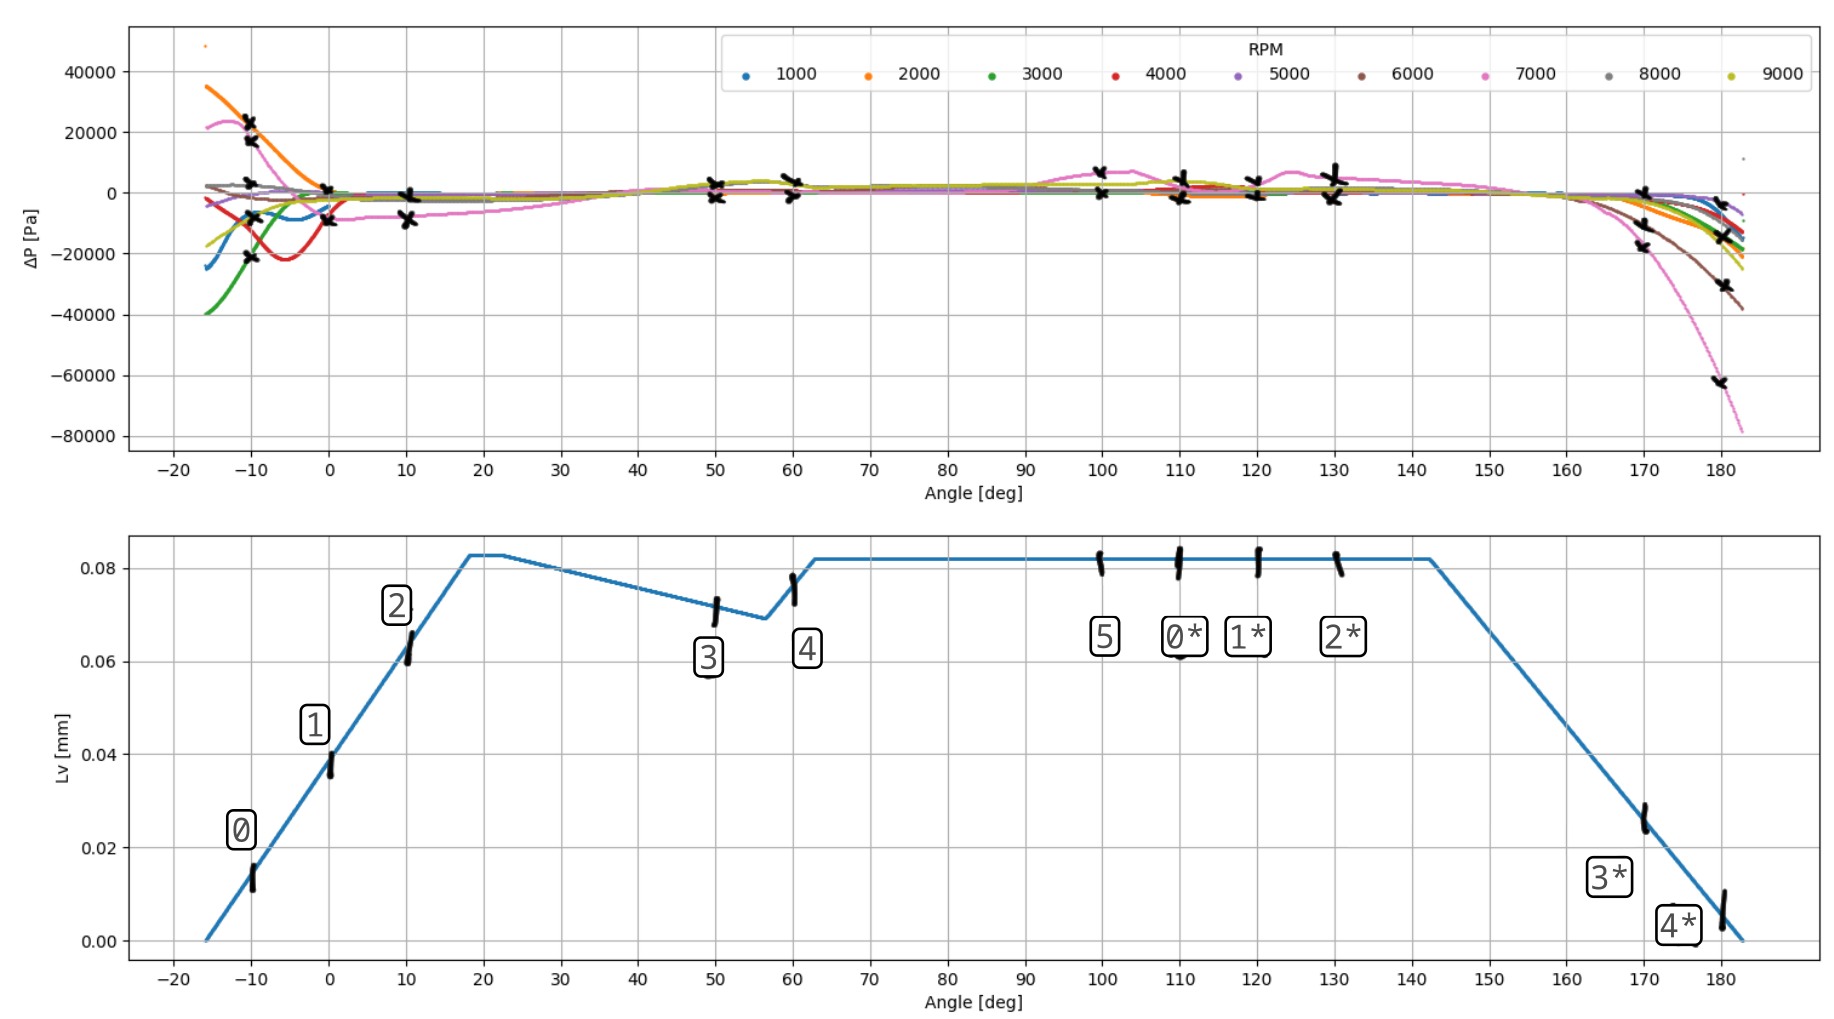
\includegraphics[width=\textwidth]{flujometrias/admision_delta_p_anot.png}
  \caption{Flujometrías puerto de admisión}\label{fig:delta_p_admision}
\end{figure}

\begin{figure}[h!]
  \centering
  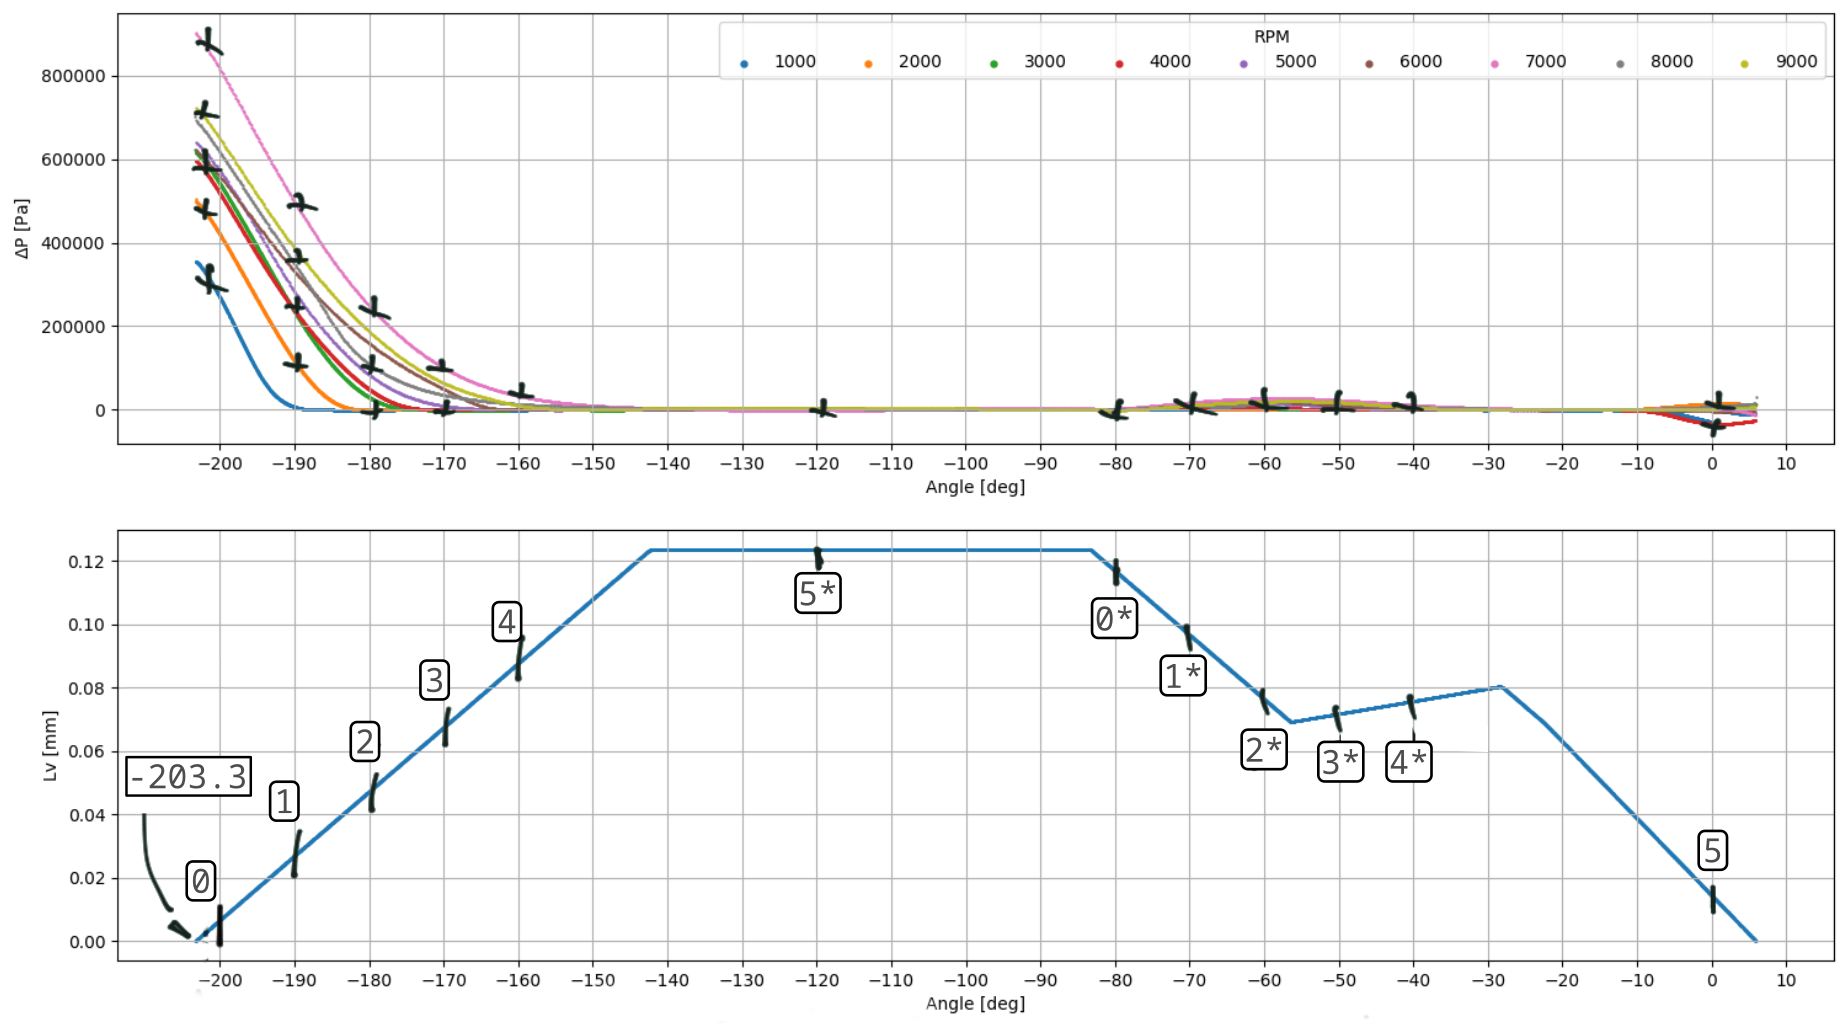
\includegraphics[width=\textwidth]{flujometrias/escape_delta_p_anot.png}
  \caption{Flujometrías puerto de escape}\label{fig:delta_p_escape}
\end{figure}


Algunas flujometrías se realizaron en tres etapas, partiendo de una malla gruesa
con celdas de $15$ mm de tamaño inicial y culminando en celdas de $5$ mm.
%
En otros se realizó directamente la flujometría con mallas base de $5$ mm.

En general se simularon alrededor de $0,02$ segundos de flujado, suficiente para
alcanzar un valor estable del caudal, como se ejemplifica en la
Figura~\ref{fig:adm_10_7000rpm}, donde se muestra el desarrollo de la simulación
en términos de $\dot{Q}$ para el puerto de admisión con el cigüeñal en
$\theta=10^{\circ}$.
%
Para esta flujometría en particular se tiene un flujo de los gases desde la
cámara hacia el puerto de admisión, correspondiente a un puerto que abre.

%
% La línea anaranjada sobre el final de la simulación representa la porción de
% datos que se seleccionó para calcular $\dot{m}$, lo cual se realizó tomando la
% media de los últimos $n$ valores obtenidos de los resultados de las flujometrías
% para los puertos de admisión y escape, las cuales se presentan en el
% Anexo~\ref{anexo:1}.
%

\begin{figure}[h!]
  \centering
  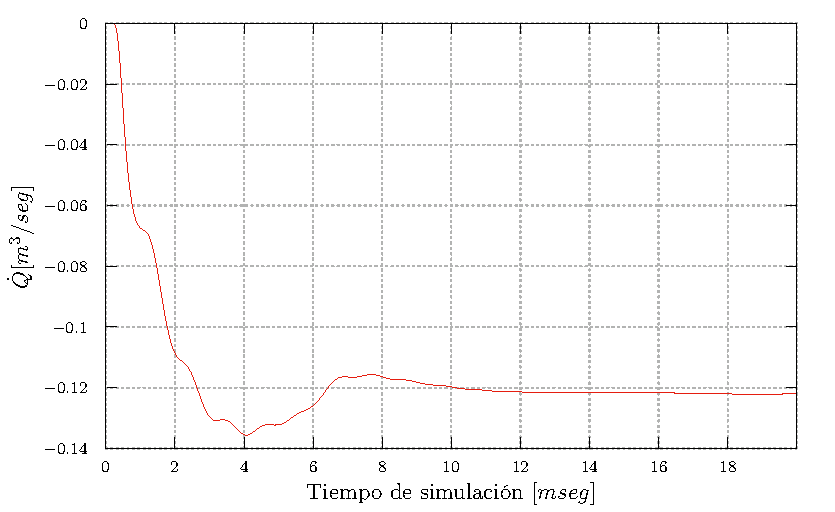
\includegraphics[width=0.7\textwidth]{./gnuplot/puerto_admision_10_7000.pdf}
  \caption{Puerto de admisión $10^{\circ}$ \@ $7000$ RPM}\label{fig:adm_10_7000rpm}
\end{figure}

Como se mencionó en la introducción del capítulo~\ref{capitulo:DESARROLLO}, la
modificación realizada a ICESym para funcionar con un mapa de $C_{D}$
dependiente de dos variables requiere que los datos de entrada estén
distribuidos en una grilla rectangular.
%
Se utilizó entonces un método de interpolación de punto más cercano suavizado
por promedio móvil con $S=2$ para generar dicha grilla a partir de los puntos
conocidos de $C_{D}$.
%
El resultado puede observarse en las Figuras~\ref{fig:mapa_cd_admision}
y~\ref{fig:mapa_cd_escape}.
%
Con respecto al gradiente de presión indicado en las figuras que se presentan en
los párrafos siguientes, para ambos puertos se define el gradiente de presión
como la diferencia entre la presión en la cámara y la presión en el puerto,
$\Delta P = P_{\text{c\'amara}} - P_{\text{puerto}}$.
%
En la Tabla~\ref{tab:resumen_puertos} se resumen los valores máximos y mínimos
de $C_{D}$ y $\dot{m}$ obtenidos para los puertos de admisión y escape.

\begin{table}[h!]
  \centering
  \begin{tabular}{cccccccc}\toprule
    Puerto   & $l_{v} [mm]$ & $\Delta P [kPa]$ & $C_{D}$ & $\dot{m} [g/seg]$ & Nota            & Figura\\ \midrule
    Admisión & 62,95        &  7,4            & 0,59   & -122              & $C_{D,\max}$     &\ref{fig:adm_cd_max} \\
    Admisión & 81,94        &  -4,95           & 0,32   &   70              & $\dot{m}_{\max}$ &\ref{fig:adm_cd_max} \\
    Escape   & 87,76        & 10,7            & 0,58   &  145              & $C_{D,\max}$     &\ref{fig:esc_cd_max}\\
    Escape   & 87,76        & 33,4            & 0,45   &  176              & $\dot{m}_{\max}$ &\ref{fig:esc_m_max}\\ \bottomrule
  \end{tabular}
  \caption{Valores máximos $C_{D}$ y $\dot{m}$ para puertos}\label{tab:resumen_puertos}
\end{table}


\subsection{Puerto de Admisión}
%
En el mapa del coeficiente de descarga para el puerto de admisión
(Fig.\ref{fig:mapa_cd_admision}) se pueden observar en rojo las zonas de menor
eficiencia del escurrimiento.
%
Esto ocurre para posiciones relacionadas con la apertura y cierre del puerto
donde las presiones y velocidades de flujo involucradas son mayores, aumentando
las pérdidas de carga.
%
La misma tendencia se observa si se representa el $C_{D}$ en función de la
apertura del puerto $l_{v}$ o del gradiente de presión $\Delta P$, ver
Figura~\ref{fig:cd_admision}.
%
Los mayores valores de $C_{D}$ ocurren para la mayor apertura o, en general,
para el menor gradiente de presión en términos absolutos.
%
También se observa que el coeficiente de descarga medio para el puerto es
aproximadamente $0,3$.

\begin{figure}[h!]
    \centering
    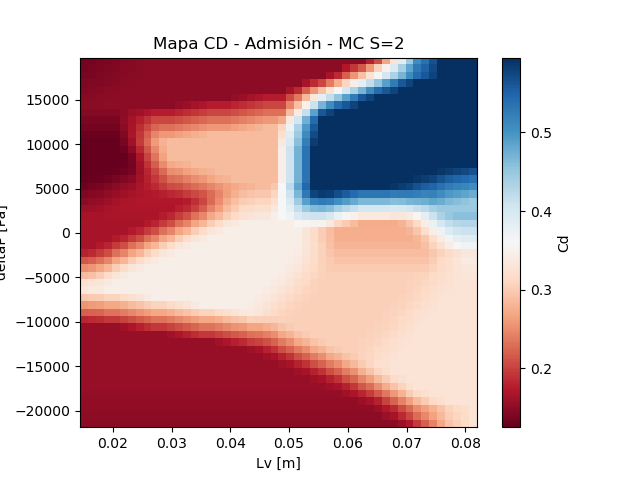
\includegraphics[width=0.7\textwidth]{mapa_cd/heatmap_cda.png}
    \caption{Mapa de $C_{D}$ del puerto de admisión}\label{fig:mapa_cd_admision}
\end{figure}

\begin{figure}[h!]
    \centering
    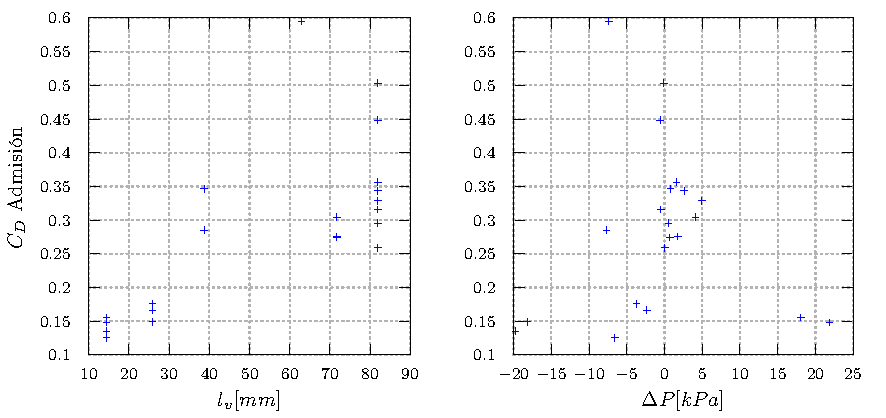
\includegraphics{gnuplot/cd_vs_alzada_adm.pdf}
    \caption{$C_{D}$ del puerto de admisión}\label{fig:cd_admision}
\end{figure}

El máximo coeficiente de descarga vale $C_{D,\max}\simeq 0,6$ para
$l_{v}=62,95 mm$ y $\Delta P\simeq +7,37 KPa$, obteniendo un flujo saliente del
puerto de $122,09 g/seg$.
%
Para este caso se observa un reflujo de gases residuales apenas abre el puerto
de admisión, correspondiendo a un ángulo de cigüeñal de $10^{\circ}$ a $7000$
RPM.


La flujometría correspondiente al último instante de la simulación se muestra en
la Figura~\ref{fig:adm_cd_max}, en la cual las líneas de corriente están
coloreadas según el módulo de la velocidad y las flechas indican el sentido de
flujo.
%
La mayor velocidad del flujo se da en el gas que sale de la cámara,
correspondiente a masa residual atrapada luego del barrido del puerto de escape.

El flujo másico máximo hacia adentro de la cámara ($\Delta P<0$) ocurre para la
misma geometría indicada en la Figura~\ref{fig:adm_cd_max}.
%
Se alcanza $\dot{m}_{\max}\simeq 70 g/seg$ para la cámara que se encuentra más
avanzada en el proceso de admisión y con máxima apertura del puerto con $l_{v}=81,94 mm$ y $\Delta P=-4,95 KPa$ siendo $C_{D}\simeq 0,32$.

\begin{figure}[h!]
    \centering
    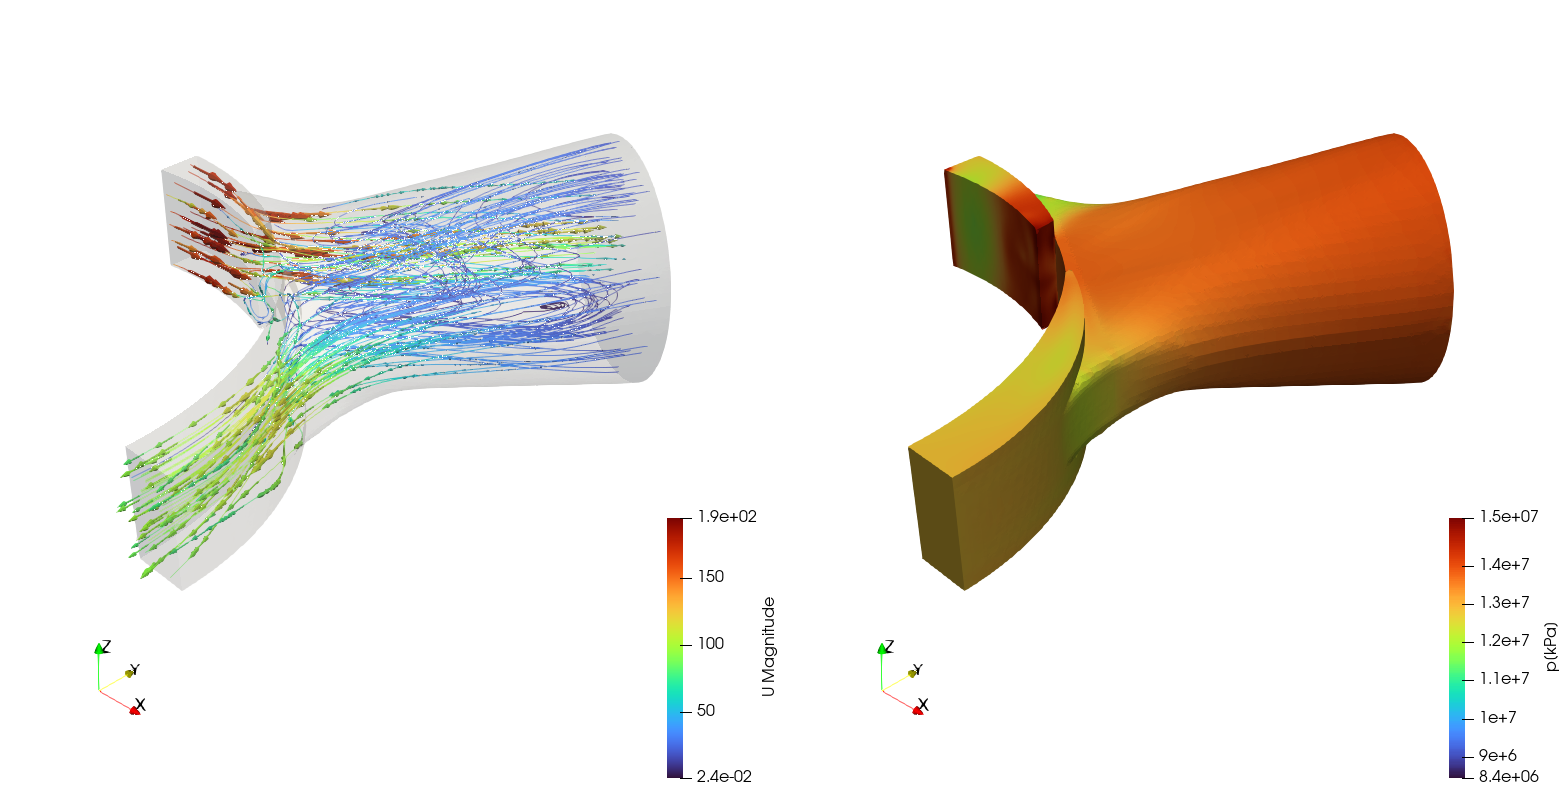
\includegraphics[width=\textwidth]{flujometrias/adm_cd_max.png}
    \caption{Admisión - Máximo $C_{D}$}\label{fig:adm_cd_max}
\end{figure}


\subsection{Puerto de Escape}
%
En la Figura~\ref{fig:mapa_cd_escape} se ilustra el mapa de $C_{D}$ obtenido para el
puerto de escape donde la tendencia es similar al puerto de admisión.
%
En la Figura~\ref{fig:cd_escape} se observa que el coeficiente de descarga es
mayor para aperturas mayores del puerto y menores gradientes de presión
($|\Delta P|\sim 0$).



\begin{figure}[h!]
    \centering
    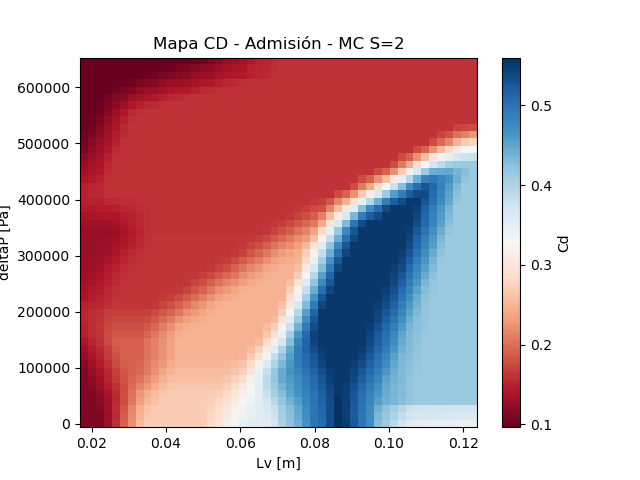
\includegraphics[width=.7\textwidth]{mapa_cd/heatmap_cde.png}
    \caption{Mapa de $C_{D}$ del puerto de escape}\label{fig:mapa_cd_escape}
\end{figure}

\begin{figure}[h!]
    \centering
    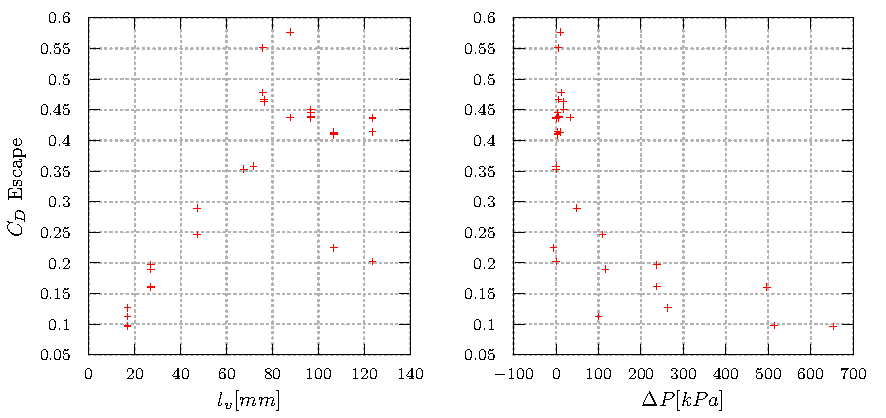
\includegraphics{gnuplot/cd_vs_alzada_esc.pdf}
    \caption{$C_{D}$ del puerto de escape}\label{fig:cd_escape}
\end{figure}

El máximo coeficiente de descarga obtenido vale $C_{D,\max}\simeq 0,58$ y ocurre
para $l_{v}=87,76 mm$, $\Delta P=10,7 KPa$ con un flujo másico de $145 g/s$
hacia afuera para $440^{\circ}$ a $9000$ RPM.
%
Por otro lado el máximo caudal másico es $\dot{m}=176,1 g/seg$ y ocurre para
$l_{v}=87,76 mm$ y $\Delta P=334 KPa$, correspondiendo a $440^{\circ}$ y 7000
RPM.
%
La flujometría correspondiente al valor máximo de $C_{D}$ se muestra en la
Figura~\ref{fig:esc_cd_max}.
%
% Las líneas de corriente muestran una gran diferencia de velocidad entre el gas
% que escapa por las paredes externas del puerto en comparación al que debe
% escurrir entre las paletas y el rotor.

\begin{figure}[h!]
    \centering
    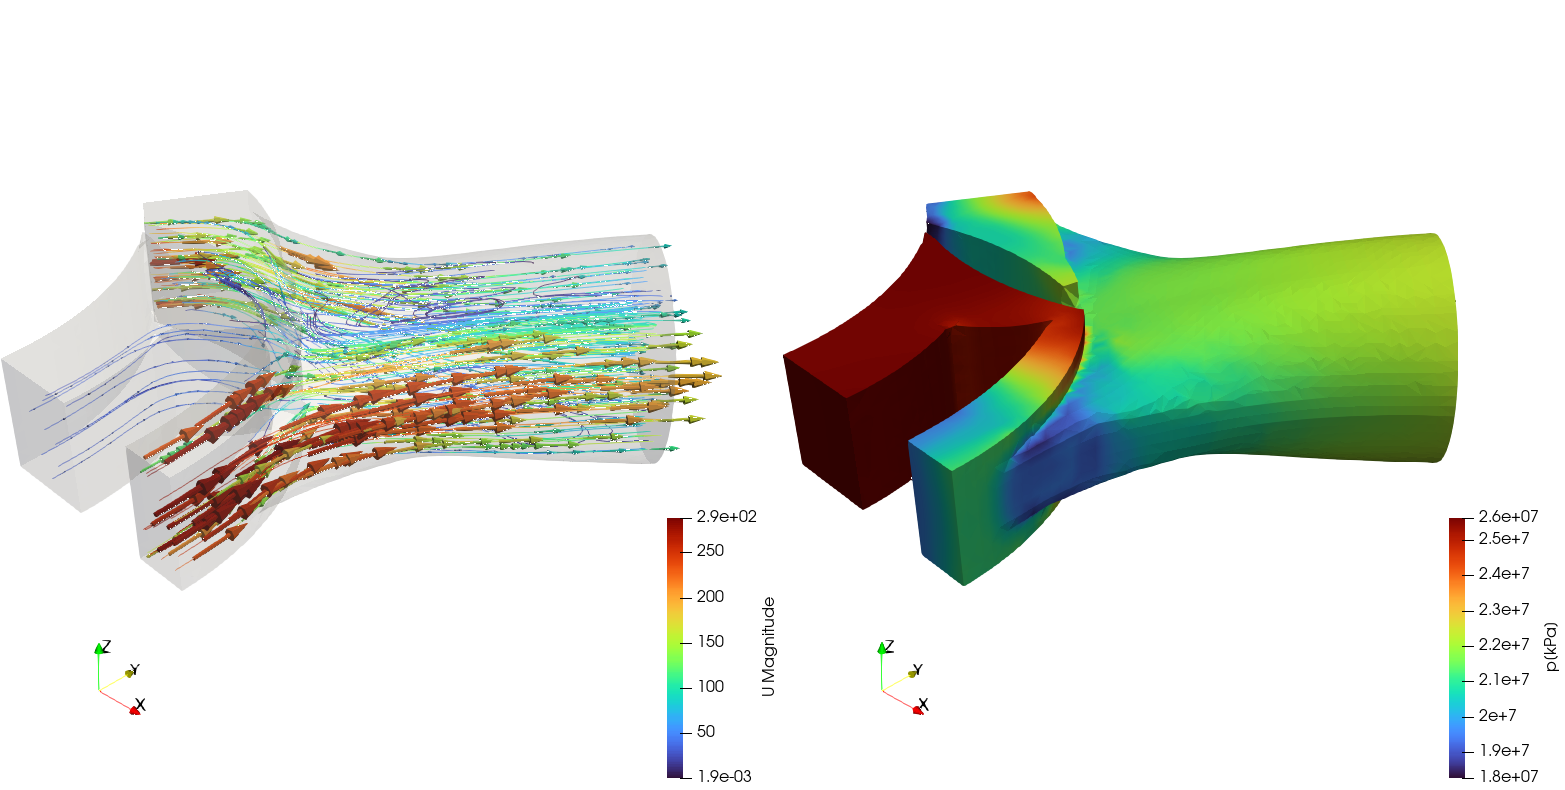
\includegraphics[width=\textwidth]{flujometrias/esc_cd_max.png}
    \caption{Escape - Valor máximo de $C_{D}$}\label{fig:esc_cd_max}
\end{figure}

La flujometría correspondiente al valor máximo de flujo másico obtenido, se
muestra en la Figura~\ref{fig:esc_m_max}.

\begin{figure}[h!]
    \centering
    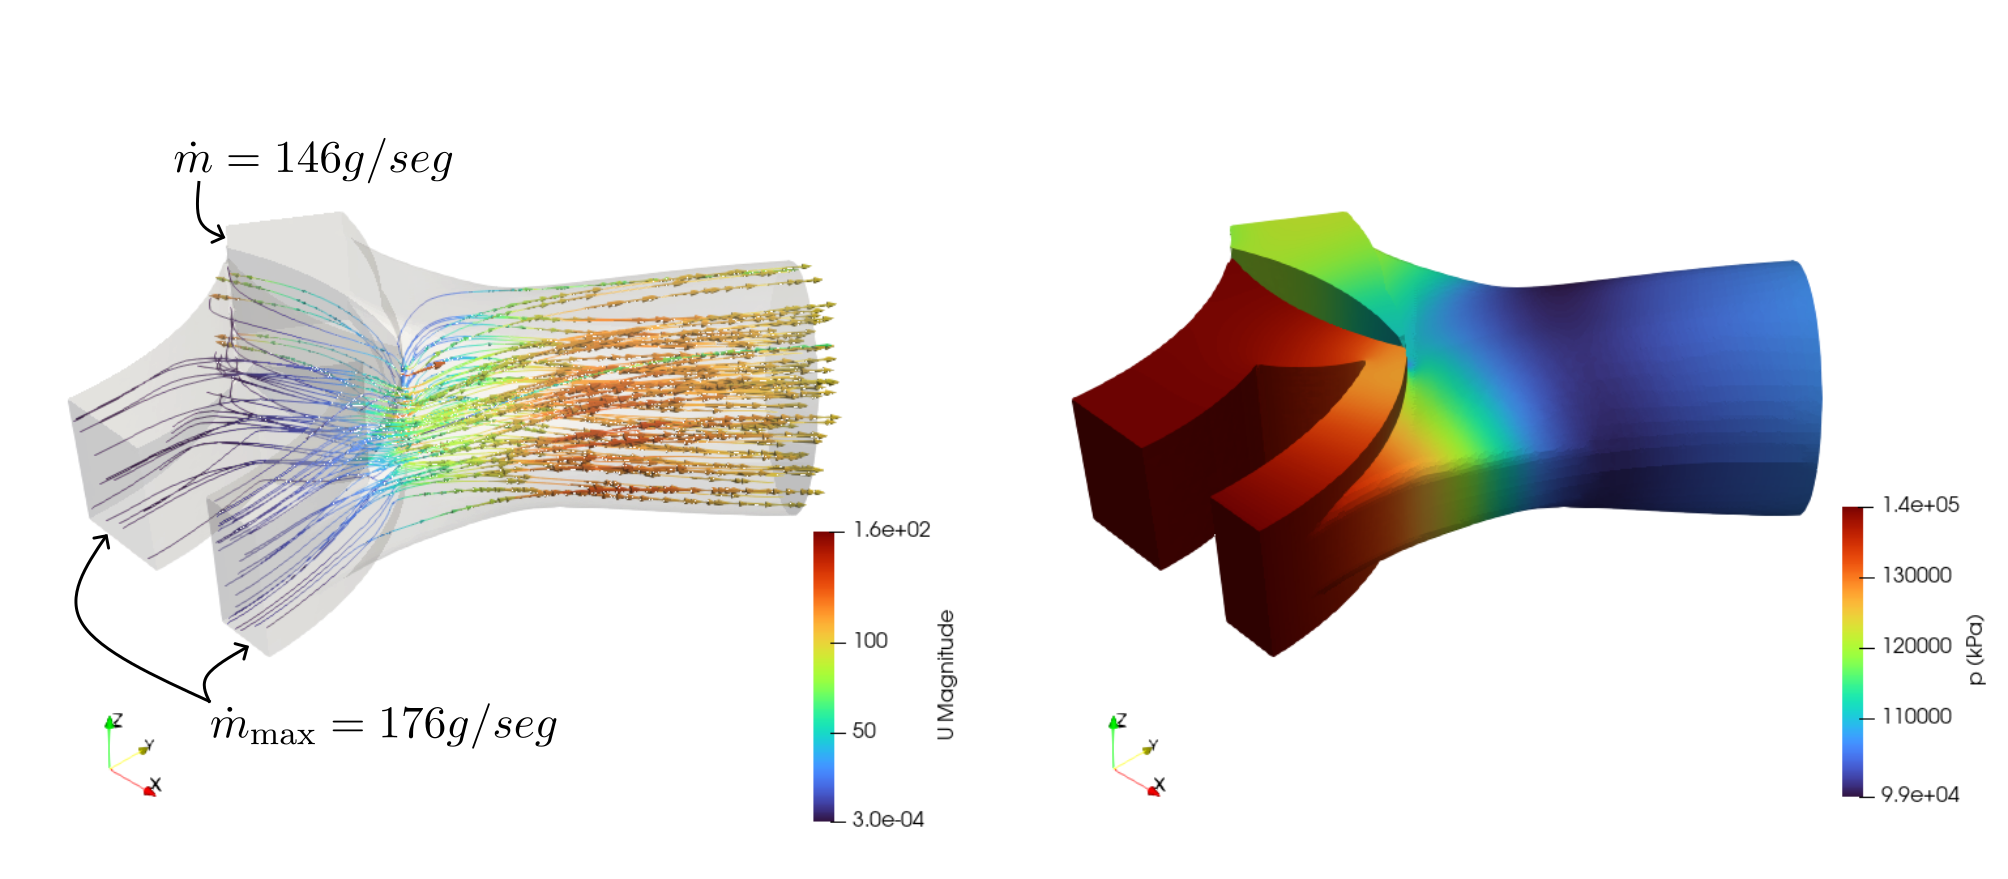
\includegraphics[width=\textwidth]{flujometrias/esc_m_max.png}
    \caption{Escape - Valor máximo de $\dot{m}$}\label{fig:esc_m_max}
\end{figure}

%%%%%%%%%%%%%%%%%%%%%%%%%%%%%%%%%%%%%%%%%%%%%%%%%%%%%%%%%%%%%%%%%%%%%%%%%%%%%%%%
%%%%%%%%%%%%%%%%%%%%%%%%%%%%%%%%%%%%%%%%%%%%%%%%%%%%%%%%%%%%%%%%%%%%%%%%%%%%%%%%
%%%%%%%%%%%%%%%%%%%%%%%%%%%%%%%%%%%%%%%%%%%%%%%%%%%%%%%%%%%%%%%%%%%%%%%%%%%%%%%%

\section{Segunda Iteración y Resultado Final}
%
En la segunda iteración se utilizó el mapa de $C_D$ para la admisión y escape
como dato de entrada de ICESym.
%
Con estos nuevos datos se realizó una serie de corridas de optimización con el algoritmo
genético, de las cuales se seleccionaron los mejores candidatos.
%
Se obtuvieron los candidatos cuyas geometrías se listan en la
Tabla~\ref{tab:2iter_geom}.
%
Los diámetros de los conductos de admisión son similares en todos los casos,
mientras que para el escape se tiene un par con conductos de 63 mm y otro con
95 mm.
%
La mayor variación ocurre en los largos de los conductos y los ángulos de apertura y
cierre.
%
Para seleccionar uno de los candidatos, se compararon las curvas de rendimiento
volumétrico, torque, potencia y fracción de gases residuales de estos motores,
las cuales se muestran en la Figura~\ref{fig:comparativa_segunda_iter}.

\begin{table}[h!]
  \centering
  \begin{tabular}{ccccccccc}\toprule
    Corrida   & DTA   & DTE & LIT   & LET   & IIA   & IFA   & EIA    & EFA \\
    -         & [mm] & [mm] & [m]   & [m]   & [gra] & [gra] & [gra]  & [gra] \\ \midrule
    run 3-4   & 99   & 63   & 0,839 & 0,79  & 3,23 & 60,0   & 78,39  & 36,29 \\
    run 5-4   & 90   & 95   & 0,742 & 0,597 & 8,39 & 60,0   & 68,23  & 23,23 \\ \bottomrule
    % run 09-04 & 82   & 91   & 0,79  & 1,758 & 3,23 & 60,97  & 75,48  & 39,19 \\
    % run 10-04 & 96   & 60   & 1,129 & 1,468 & 6,13 & 66,78  & 62,42  & 40,65 \\ \bottomrule
  \end{tabular}
  \caption{Geometrías de segunda iteración}\label{tab:2iter_geom}
\end{table}

\begin{figure}[h!] \centering
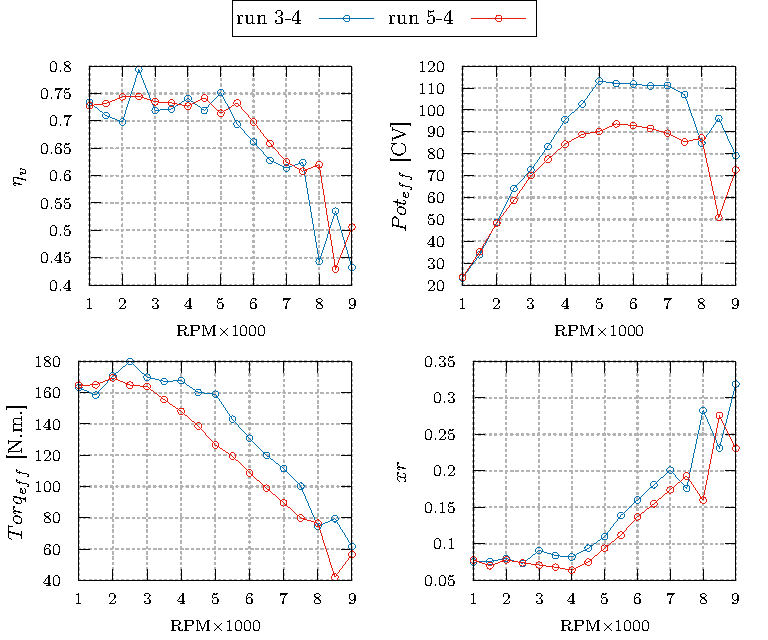
\includegraphics[width=\textwidth]{gnuplot/comparativa_segunda_iter_mep.pdf}
  \caption{Comparativa de candidatos} \label{fig:comparativa_segunda_iter}
\end{figure}

En base a esta comparativa se optó por seleccionar la corrida denominada como
``run 3-4''

% , este motor presenta un máximo de torque y potencia en 2500 RPM,
% también presenta una curva de rendimiento volumétrico suave con un máximo en
% 2500 RPM.
%
% En términos de potencia mantiene valores elevados a partir del cercanos a los
% 130 CV.
%
En todos los candidatos se observa una alta fracción de gases residuales a altas
RPM y una disminución notoria del rendimiento volumétrico.

El motor tiene una potencia máxima de 113 CV a las 5000 RPM que se mantiene
plana hasta las 7000 RPM.
%
En cuanto al par motor, se tiene el máximo de 180 Nm a 2500 RPM y se mantiene
por encima de 160 Nm hasta las 5000 RPM.
%
Este coincide con el máximo de rendimiento volumétrico de $\sim 0,845$.
%
En la Figura~\ref{fig:PoTi_segunda_op} se notan los efectos del coeficiente de
descarga en la simulación del motor, comparando los resultados de la primera
iteración con coeficientes de descarga constantes a la segunda con el mapa de
$C_{D}$ en función de la presión y grado de apertura del puerto.

\begin{figure}[h!]
  \centering
  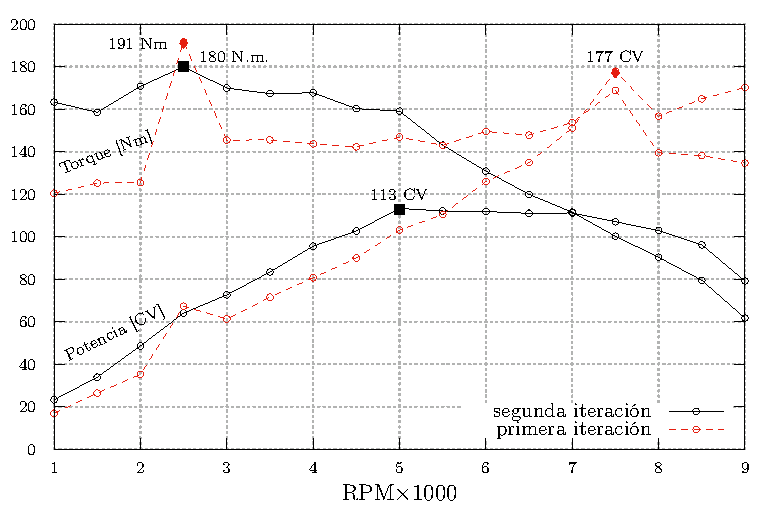
\includegraphics{gnuplot/comparativa.pdf}
  \caption{Comparativa de Torque y potencia al freno} \label{fig:PoTi_segunda_op}
\end{figure}
